\documentclass{acm_proc_article-sp}
\newcommand\floor[1]{\lfloor#1\rfloor}
\newcommand\ceil[1]{\lceil#1\rceil}
\newcommand{\tabitem}{~~\llap{\textbullet}~~}
\usepackage{textcomp}
\usepackage{url}
\usepackage{algorithm}% http://ctan.org/pkg/algorithms
\usepackage[noend]{algpseudocode}
\usepackage{pifont}
\usepackage{tabulary}
\usepackage{amsmath}
\usepackage{float}
\usepackage{cleveref}
\usepackage{caption}
\DeclareCaptionType{copyrightbox}
\usepackage{subcaption}
\usepackage{pgfplots}
\DeclareMathOperator*{\argmax}{argmax}
\newcommand*{\argmaxl}{\argmax\limits}
\newcommand{\norm}[1]{\left\lVert #1 \right\rVert}
\begin{document}
\title{Who to query? \\A two stage querying algorithm for tracking variant/unknown event distributions }
\numberofauthors{3} %  in this sample file, there are a *total*
\author{
% You can go ahead and credit any number of authors here,
% e.g. one 'row of three' or two rows (consisting of one row of three
% and the second row of one, two or three).
%
% The command \alignauthor (no curly braces needed) should
% precede each author name, affiliation/snail-mail address and
% e-mail address. Additionally, tag each line of
% affiliation/address with \affaddr, and tag the
% e-mail address with \email.
%
% 1st. author
\alignauthor
Mai ElSherief\\
   \affaddr{Dept. of Computer Science }\\
   \affaddr{UC Santa Barbara}\\
  %\affaddr{Santa Barbara, CA}\\
   \email{mayelsherif@cs.ucsb.edu}   
   \alignauthor
Ramya Raghavendra\\
   \affaddr{IBM T. J. Watson Research Center }\\
   \email{rraghav@us.ibm.com}
% 2nd. author
\alignauthor
Elizabeth Belding\\
  \affaddr{Dept. of Computer Science }\\
   \affaddr{UC Santa Barbara}\\
   %\affaddr{Santa Barbara, CA}\\
   \email{ebelding@cs.ucsb.edu}
}
\maketitle
\begin{abstract}
In this paper, we propose a two-stage node selection algorithm for resource constrained systems based on the nodes location to track incidents in a $2D$ environment. Our algorithm maximizes the dispersion of the locations with a portion of the available resources. Based on the nodes' sensing feedback, it selects the K nearest neighbors for the nodes that provide a positive feedback using the rest of the available resources. We test the two-stage algorithm on three different distributions: uniform, clustered and long-tailed. We then apply the algorithm to a real harassment dataset provided by Hollaback. The proposed algorithm outperforms a random selection policy by up to $63\%$ and a policy that relies on dispersion maximization without incorporating feedback from the nodes by up to $68\%$.
\end{abstract}
%\category{H.1.2}{User/Machine Systems}{Human information processing}
%\keywords{Street harassment, Urban analysis, Walkability score, Transit Score, Transit route }
\section{Introduction}
Sensors have become an integral part of daily life. The common smartphone includes a variety of different sensors, such as camera, microphone, GPS, accelerometer, digital compass, light sensor, and Bluetooth as proximity sensor. The ubiquity of sensors is also prevalent in the urban environment. Examples include traffic sensors, agriculture sensors, wireless parking sensors, infrastructure sensors, weather, and pollution sensors. Data analysis of such sensors can hold important observations. For instance, ~\cite{ferreira2013visual} leverages the geographic and temporal data associated with taxis in NYC to gain insight into many different aspects of city life, from economic activity and human behavior to mobility patterns. When combined with crowdsourcing of humans senses, critical data can be generated about surroundings. One example is the application ``Waze'', where users can report traffic jams, accidents and other road related incidents in real-time. The work in~\cite{agapie2015crowdsourcing} uses local workers to collect data at events and remote workers to curate the collected information and generate event reports.\par

Despite the ubiquity of human and device sensors, the challenges of energy preservation and resource constraints are always present. The truth is that all systems are bound by a fixed amount of resources. For instance,~\cite{marco2003many} and~\cite{pattem2008impact} focus on eliminating redundancies among correlated sensor measurements. \par

In this paper, we investigate the problem of how we can probe a limited subset of sensors in a particular environment to either preserve energy or other resources. In particular, we envision a world where users/sensors can be probed to collectively answer some question. An unanswered question can be related to a phenomenon that needs to be tracked under the constraints of $N$ resources. The experiments, analyzing the spatial and temporal characteristics of the twitter feed activity responding to a 5.8 magnitude earthquake which occurred on the East Coast of the United States (US) on August 23, 2011 in~\cite{crooks2013earthquake}, support the notion that people act as sensors to give us comparable results in a timely manner. Examples of resource constrained systems include disaster and safety applications or in general terms to track any spatial phenomenon. In an emergency, communication networks tend to fail and available resources, such as bandwidth, are scarce~\cite{manoj2007communication}. Under these constrained settings, the two-stage algorithm can be used to probe the crowd/sensors about the current situation of the disaster in their current location. Another example of safety applications is what happens in Tahrir Square during Egyptian revolutions in 2011 and 2012. At that time, women were discouraged from participation due to the high harassment rates~\cite{guardianSH}. This resulted in movements of men forming protective human shields~\cite{worldPostHS} around female protestors to avoid assault. Our proposed algorithm can be used to query users for safe zones for women and then use the results for safe routing around the square or for identifying zones where women can safely participate in the protests. \par
Our contribution in this paper is three-fold. First, we propose a two-stage matching algorithm that probes/queries $N$ nodes out of $M$ available nodes to track a real-time phenomenon with no prior information about the event distribution. The algorithm outperforms the random user selection by up to $63\%$ in terms of choosing nodes chosen that are closer to the events and outperforms the dispersion maximization algorithm by up to $68\%$. Secondly, we study the performance of our proposed algorithm under three different distributions: uniform, clustered and long-tailed. We then test the algorithm on a real dataset that is comprised of harassment cities in three different cities. Third, we discuss how the algorithm can be altered based on trust variations and prior knowledge availability.\par
The rest of this paper is organized as follows. Section 2 surveys the related work while Section 3 describes the proposed two-stage algorithm. Section 4 experimentally evaluates the proposed algorithm, and Section 5 discusses tradeoffs and variations of the two-stage algorithm. Section 6 concludes the paper.
\section{Related Work}
Since the introduction of ``crowdsourcing'' as a modern business term in 2006~\cite{howe2006rise}, a significant body of work has been dedicated to the study and implementation of crowdsourcing in real life applications. In particular, spatial crowd sourcing, where crowd participation is bound by a particular geographic area, has received significant attention~\cite{kazemi2012geocrowd, deng2013maximizing, yu2015quality}. For instance, ~\cite{liu2013using} introduces a location-based real-time social question answering service, where users can ask temporal and geo-sensitive questions and then receive answers that are crowdsourced in a timely fashion. A crowdsensing platform was introduced in~\cite{cardone2013fostering} to facilitate the collaboration of large groups of people participating in collective actions of urban crowdsourcing.\par

Using people as sensors, collective sensing and citizen science have opened doors for interesting research problems. Some of these challenges are introduced in~\cite{blaschke2011collective}. One important challenge in geo-crowd sensing is detecting unusual events. The work proposed in~\cite{lee2010measuring} leverages microblogging websites such as Twitter to detect unusual geo-social events by identifying unusually crowded regions. Another challenge is the refinement of crowd sensed data and detection of fake data. Solutions based on a user's history and reputation have been introduced in the literature. The work in~\cite{yu2013reputation} proposes a reputation-aware model that balances the workload between users. Another challenge is fusing untrustworthy estimates~\cite{venanzi2013trust}. Taking into account spatial properties, ~\cite{venanzi2013crowdsourcing} tackles the problem of merging multiple spatial observations reported by possibly untrustworthy users using a heteroskedastic Gaussian process model.\par

Another related body of work is sensor networks~\cite{akyildiz2002survey} that include spatially and ubiquitously distributed autonomous sensors used to monitor physical and environmental conditions. Since the sensors are typically small, low-powered nodes, resource-constrained protocols emerged to preserve the energy of these devices. Examples of work targeting energy preservation include, but are not limited to~\cite{sallai2004acoustic}, where the authors achieve geographic localization using noise tolerant acoustic ranging mechanism to meet severe resource constraints. In~\cite{krishnamachari2002impact}, data aggregation methods were introduced and achieved significant performance gains in comparison to end to end routing. The work proposed in~\cite{fontugne2013strip} implements a system that analyzes sensor behaviors and uncovers misbehavior corresponding to inefficient device usage that leads to energy waste. In contrast, our work focuses on the how to choose sensors to query based on their location while constraining the number of probes to a portion of the total number of sensors hence, preserving energy.



\section{Research question and proposed algorithm}
In our system, we have a two-dimensional grid and a number of objects that can sense the environment around them. These objects can be humans, artificial sensors, mobile phones or even robotic sensors. We are interested in answering the following question: "What is the answer to Question X in this grid?". To find the answer, one approach would be to query all the objects in the two-dimensional space and aggregate the findings. However, in certain situations like in the case of an emergency, the network's performance degrades and preserving energy and other resources become critical~\cite{manoj2007communication}. In this paper, we investigate how to answer the aforementioned question in the case of limited resources. Hence, the question becomes: \textit{Given $N$ resources, who should you select to track a phenomenon?}\par


If we attempt to tackle this question from a probabilistic point of view, then the straightforward answer is to try to select objects with the same probabilistic distribution as the phenomenon. For instance, if we know that a certain phenomenon occurs at different places in the two-dimensional grid uniformly, then we would have no bias in selecting the users to query, i.e. each user/object should have the same probability of selection to be queried. On the other hand, if we know the phenomenon we are interested in is more prevalent in certain areas of the grid as opposed to other areas, we should take that into consideration when we are selecting the users such that we query users in the area of interest and fewer users in areas where there is a smaller probability of occurrence.\par

The question becomes far more challenging if the distribution is not known or if it is time variant. In this case, we inquire if there is a systematic algorithm that can be used for querying/selecting users to track a phenomenon regardless of the probabilistic distribution or time variation. In the following sections, we propose a two-stage algorithm that queries objects without any assumptions about the distribution of events and succeeds in locating objects that are close to the events and in covering up to more than $80\%$ of the incidents. \par

\subsection{Technique Description}
We assume that there are $M$ users in a two-dimensional grid and that the system that selects a user to query is bounded by $N$ resources, where $N < M$.  Each of the $M$ users has a specific location in the grid, determined by a two-dimensional system, e.g. (x, y) or a (lat, long). We also assume that the selected users will fully cooperate and respond to the query. If needed, a pre-selection phase can be used to eliminate users that are not likely to co-operate, such as requiring the installation of an app to facilitate querying. Here, we focus on how to select $N$ out of $M$ users, where $N < M$ to keep track of events occurring in the two-dimensional grid.\par

Our technique combines querying users to maximize the dispersion of their location in the grid with $K$ nearest neighbor (KNN) selection as depicted in Algorithm~\ref{TSalgorithm}. We divide the selection of users into two stages. In the first stage, our goal is to select users that maximize the dispersion of users' locations. This is accomplished by selecting the set of points that maximizes the average distance between each point and its nearest neighbor as follows:
\begin{equation} \label{eq:maxDisp}
\argmax \sum_{i=1}^{\floor{(FSP*N)}} \norm{p(i) - NN(p(i))}^2
\end{equation}
\begin{algorithm}
\caption{Two-stage querying algorithm}
\label{TSalgorithm}
 \begin{algorithmic}[1]
     \Function{selectUsersFromGrid }{$FSP, N$}
         \State selectedUsers = $\left\{\right\}$
         \State firstStageCnt = $\floor{(FSP*N)}$
         \State secondStageCnt = $M - firstStageCnt$
         \State firstStageUsers = maximizeDisp(firstStageCnt)
         \State usersFeedback = feedback(firstStageUsers)
         \If {usersFeedback.size == 0}
                \State selectedUsers = maximizeDisp(secondStageCnt){}
         \Else
             \State {selectedUsers.append(firstStageUsers)}
         \EndIf 
       \State firstStageQuota = calculateQuota(firstStageUsers)
       \For{$user_i$ in firstStageUsers}
     \State selectedUsers.append(KNN($user_i$, $firstStageQuota_i$))
   \EndFor
\State return {selectedUsers}
\EndFunction
\end{algorithmic}
\end{algorithm}


where $p$ represents a point in the $2D$ grid and $NN$ represents the nearest neighbor; the distance is measured as the Euclidean distance. The algorithm attempts to maximize the dispersion with a percentage of the $N$ resources up a certain number of trials controlled by the ``maximization trials'' setting as explained in Table~\ref{table:systemParameters}. \par
After the dispersin maximization phase, we query the sensors that were selected and look at the feedback of these sensors. The feedback provided is application dependant. For some applications, the query can be in the form of probing for measurement and if that measurement exceeds a certain threhold, the system marks this as a positive feedback of the incident under investigation. In other applications such as in the case of emergency sitiuations, the query is usually a simple yes-no question. An example is in~\cite{crooks2013earthquake}, when an earthquake occured at the East Coast in the US in 2011, the query was the question ``Did You Feel It?'' (DYFI). Based on the senors/objects feedback in the first stage, we then proceed to a more fine-grained selection. The objects that provide a positive feedback, where the definition of a positive feedback is application dependant, are called the \textit{pivot users}. In our experiments, we simulate the positive feedback. A node will provide a positive feedback if it is in the kNN of one or more incidents in the grid. The positive feedback does not contain any information about the number or location of incidents. In the second stage, we divide the rest of the resources among the nearest neighbors for each of the pivot users. If no nodes provide a positive feedback, the second stage maximizes the dispersion of the location of nodes with the rest of the available resources. \par

This initial algorithm assumes that the first stage users will respond with unfalsified responses. To relax this assumption, we explore dividing the selection of the second phase users into two groups: a group that consists of the $KNN$ of trusted pivot users, and another group that aims to maximize the dispersion. In the next section, we focus on studying our two-stage querying algorithm with the assumption of having full trust in the crowd and discuss other variants of the technique in Section 5.\par

\begin{table}{}
\centering
\begin{tabulary}{0.5\textwidth}{|L|}
\hline
\textit{Environment settings: }\\
\tabitem matrix dimension: the length and width of the $2D$ spatial matrix. We model the spatial area under investigation as a $2D$ square matrix.\\
\tabitem incident count: number of incidents distributed across the cells of the spatial matrix\\
\tabitem resources or crowd count: the $M$ resources from which $N$ will be chosen to query, where $N < M$.\\
\hline
\textit{Query settings:}\\
\tabitem $N$: the number of resources the system is limited by to query/sense \\
\tabitem first stage percentage (FSP): the percentage of users/sensors of the $N$ resources that will be selected to query in the first phase. In our analysis, we test the cases of selecting $20\%, 40\%, 60\%$ and $80\%$ of the $N$ resources in the first stage.\\
\tabitem k setting: used to identify the KNN crowd individuals/sensors to an incident\\
\hline
\textit{Approximation settings: }\\
\tabitem maximization trials: number of attempts to maximize the dispersion of selected individuals/sensors from the crowd\\
\hline
\end{tabulary}
\caption{Parameters of the two-stage querying algorithm.}
\label{table:systemParameters}
\end{table}

\section{Experiments}
To quantify the performance of our technique, we perform multiple experiments with three types of data spread: clustered, uniform and real datasets. In our experiments, we compare our algorithm in the selection of users to two alternative approaches as follows:
\begin{itemize}
\item Random user selection: For this approach, we select $N$ users randomly based on a uniform distribution.
\item Dispersion maximization (DispMax) selection: In this approach, $N$ users are selected from the resources/crowd who maximize the dispersion of their locations.
\end{itemize}
\subsection{Experiment variables}
There are multiple variables that can be controlled to test the behavior of the two-stage querying technique. Table~\ref{table:systemParameters} summarizes the most important.
The environment settings are related to the size of the $2D$ matrix, the number of incidents, the distribution of incidents across the matrix, and the number of resources from which to choose. In all of our experiments, except the case study, we set up the $2D$ matrix as a $10$ by $10$ matrix. We show results for incident count of $50$ and number of resources ($M$) of $100$. 
We varied the environment settings in our experiments and we do not observe any differences in performance. Instead, we focus on varying the query settings to better understand the two-stage technique. In this section, we vary the first stage percentage and leave the variation of the $k$ setting to the following section. We also show results for $t\_setting = 30$, which constitutes $30\%$ of the available resources ($M$). We notice that the gap between the performance of our technique and the other techniques increases when $t\_setting$ decreases, and all the techniques converge in performance when $t\_setting$ approaches $M$. \par

We compare the performance of our technique to two alternative selection approaches: random selection and dispersion maximization. To do so, we utilize two different metrics: count of nodes queried in the $KNN$ of incidents, and the number of incidents covered by the nodes queried. The two metrics are defined as:
\begin{itemize}
\item Close node count: the absolute number of sensors/resources in the KNN of each incident for all incidents. This is formally represented as follows:
\begin{equation}
Close\ node\ count = \sum \forall_{incident\ i}\ |(KNN_i \cap {QU})|
\end{equation}
where $QU$ (the ``Queried Users'' set) is the set of users selected for querying.
\item Coverage: the number of incidents covered out of the total number of incidents occurring in the $2D$ matrix. We define an incident as covered if at least one of the nodes in the incident's KNN was queried. This is formally measured as:
\begin{equation}
Coverage = \sum \forall_{incident\ i}\ Coverage_i\  where,
\end{equation}
\[
 Coverage_i =
\begin{cases}
 1,& \text{if }(KNN_i \cap {QU}) \neq \phi\\
 0,              & \text{otherwise}
\end{cases}
\]
\end{itemize}
\subsection{Clustered data experiments}
Geographer Waldo R. Tobler's stated in the first law of geography: ``Everything is related to everything else, but near things are more related than distant things.'' In this subsection, we assume that the incidents are related to each other in a clustered way, i.e. they form clusters across the $2D$ spatial matrix as seen in Fig~\ref{fig: clust}. Our goal in this section is to study the performance of the different approaches when the events are clustered.\par
\begin{figure}[!h]
\centering
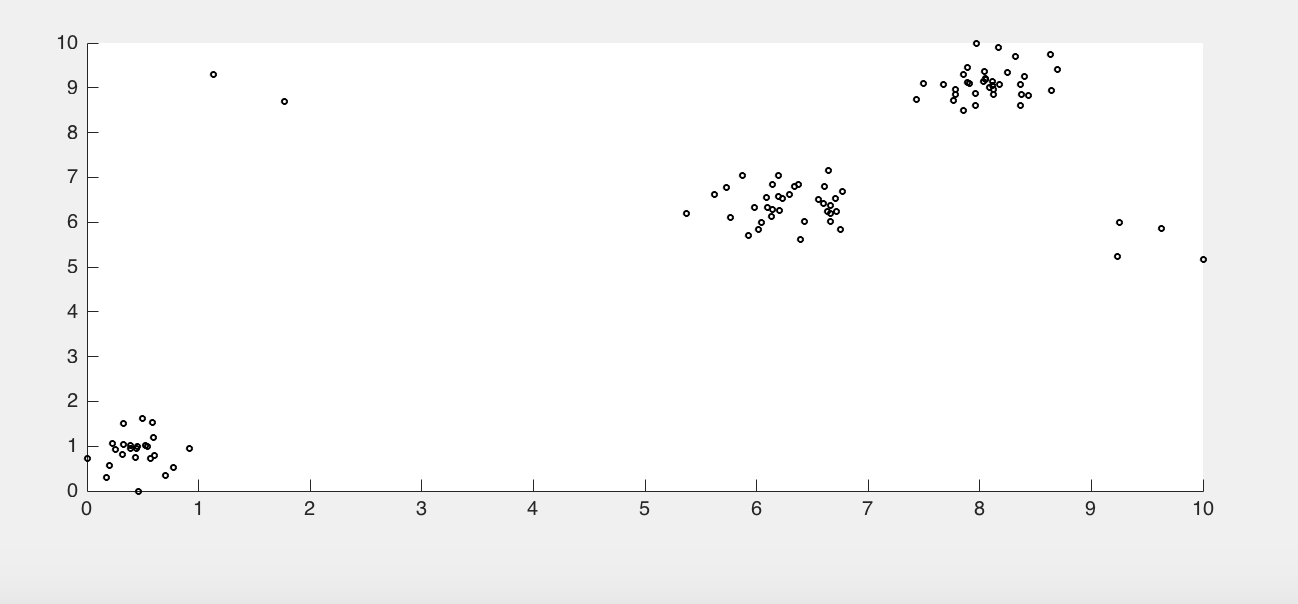
\includegraphics[width=9cm ,height=5.5cm]{figuresPng/clust.png}
\caption{An example of a $2D$ spatial matrix with $5$ clusters.}\label{fig: clust}
\end{figure}

For this set of experiments, we vary the number of clusters in our $2D$ matrix from one to ten clusters while fixing the resources or crowd count to be $100$. To enforce data variability, we model the size of each cluster as a random variable while ensuring that the aggregated size of all the clusters is equal to the crowd count. For each case of number of clusters, we average over $100$ different configurations. Our objective is to measure the effect of variation of the first stage percentage on our performance metrics.\par

Figure~\ref{fig:clusteredResults} depicts the results for Close node count when varying the first stage percentage (FSP) from $20\%$ to $80\%$. The two-stage querying technique always outperforms the Random node selection and the Dispersion Maximization selection. Table~\ref{table:clusteredSurge} depicts the surge in Close node count in comparison to the Random and Dispersion maximization techniques. As the amount of resources queried in the first stage decreases, the close node count increases. This is due to the fact that when the first stage percentage decreases, the second stage resources increase under limited resources constraints, which focuses on resources close to incidents detected in the first stage. On the other hand, incident coverage tends to increase as the first stage count increases. This is depicted in Figure~\ref{fig: clustCoverage}. Both Close node count and Incident coverage tend to increase with the number of clusters until the number of clusters is around four or five. Then, they decrease.

%Real life examples of clustered events include
%- Begin by pointing out real-life examples of spatially clustered phenomenon and spatial correlation in general. Lots of social phenomena are spatially dependent. %(https://books.google.com/books?id=jbFRojt85TUC&pg=PA2&lpg=PA2&dq=clustered+phenomena&source=bl&ots=yftMfShveB&sig=XcPOJriI1gineu-%A2YGpoJT3OII&hl=en&sa=X&ved=0ahUKEwiBp4a-s-zKAhUI5WMKHZQ3Cd8Q6AEITzAI#v=onepage&q=clustered%20phenomena&f=false)
\begin{figure}[!h]
\centering
\subcaptionbox{Close node count with $FSP = 20\%$ of available resources. \label{fig: clust_20}}{%
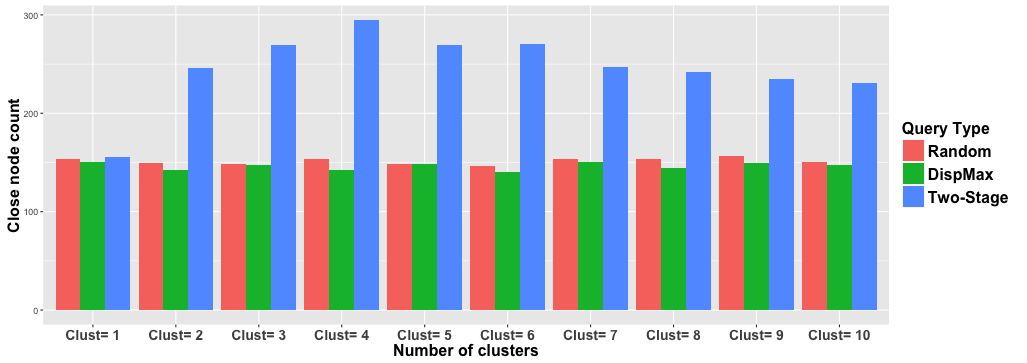
\includegraphics[width=9cm, height=4.5cm]{figuresPng/fsTwentyPerc.png}%
}\par\medskip
\subcaptionbox{Close node count with $FSP = 40\%$ of available resources. \label{fig: clust_40}}{%
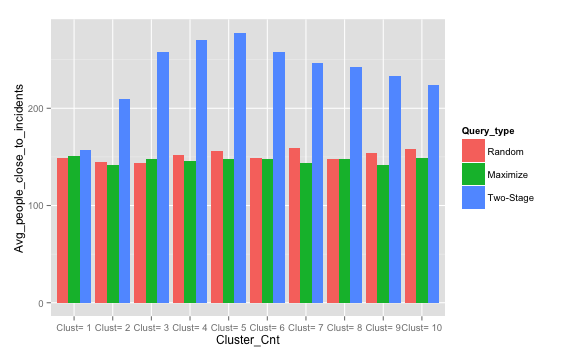
\includegraphics[width=9cm, height=4.5cm]{figuresPng/fsFourtyPerc.png}%
}\par\medskip     
\subcaptionbox{Close node count with $FSP = 60\%$ of available resources. \label{fig: clust_60}}{%
  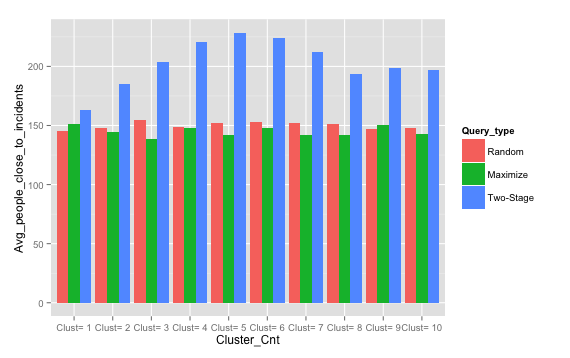
\includegraphics[width=9cm, height=4.5cm]{figuresPng/fsSixtyPerc.png}%
}
\subcaptionbox{Close node count with $FSP = 80\%$ of available resources. \label{fig: clust_80}}{%
  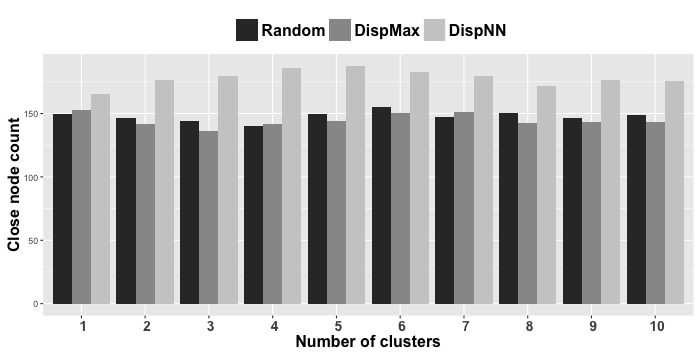
\includegraphics[width=9cm, height=4.5cm]{figuresPng/fsEightyPerc.png}%
}
\caption{Average number of nodes close to the incidents (Close node count) as FSP varies.}
\label{fig:clusteredResults}
\end{figure}


\begin{figure}[!h]
\centering
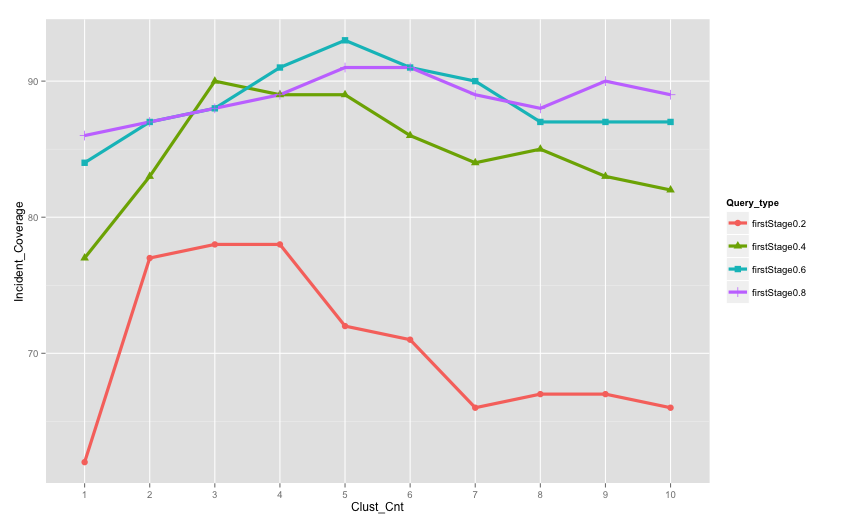
\includegraphics[width=9cm ,height=5.5cm]{figuresPng/Coverage_Result.png}
\caption{Incident coverage for different values of First stage percentage. }
\label{fig: clustCoverage}
\end{figure}

\begin{table}[!h]
\centering
\begin{tabulary}{0.5\textwidth}{|C|C|C|C|C|}
\hline
First stage percentage & $20\%$ & $40\%$  & $60\%$  & $80\%$  \\ \hline
Surge over Random   & $62.5\%$ & $58.89\%$  & $35\%$  & $20\%$  \\ \hline
Surge over Dispersion Maximization   & $67.8\%$ & $62.32\%$  & $39.8\%$  & $20.64\%$ \\ \hline
\end{tabulary}
\caption{Surge of Two Stage technique in comparison to Random and Dispersion Maximization techniques.}
\label{table:clusteredSurge}
\end{table}
\begin{figure}[!h]

\subsection{Uniformly distributed data experiments}
The next step of experiments, the probability of occurrence of incidents is uniform across the grid, i.e. $P_I (j) = P_I (k)$ where $j \neq k$ and $P_I$ denotes the probability of an incident occurring at a specific cell. We randomly generate $100$ different matrices and average the results. We note that if we know that the distribution of the incidents is uniform, the best we can do is to choose $N$ nodes uniformly. Using the two-stage technique, we select $N$ nodes without assuming any distribution about the incidents and check the performance in comparison to the uniform random selection, which yields the best results in terms of close node count. Figure~\ref{fig:uniClosePeople} shows that the two-stage technique with $FSP = 20\%$ achieves the highest number of close node count while Figure~\ref{fig:uniIncdCove} shows that the two-stage technique with $FSP = 80\%$ achieves higher coverage that the uniform random policy and it is close to the maximum coverage by an average of $1.32$ incidents. This shows that our technique can achieve better node selection than the uniform scheme in terms of close node count when $FSP = 20\%$ and achieves better coverage than the uniform scheme in $FSP = 80\%$.

\centering
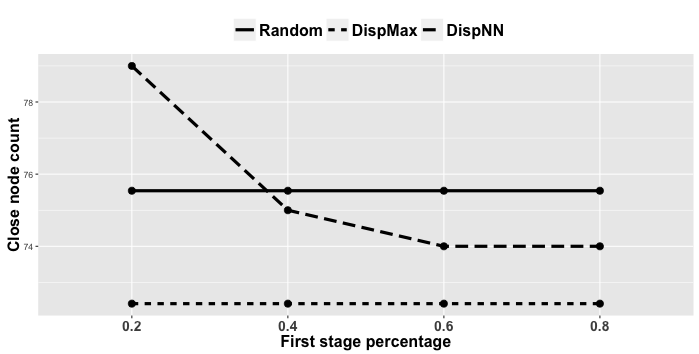
\includegraphics[width=9cm ,height=5.5cm]{figuresPng/Uni_ClosePeople_Count.png}
\caption{Close node count for different values of First stage percentage. }
\label{fig:uniClosePeople}
\end{figure}
\begin{figure}[!h]
\centering
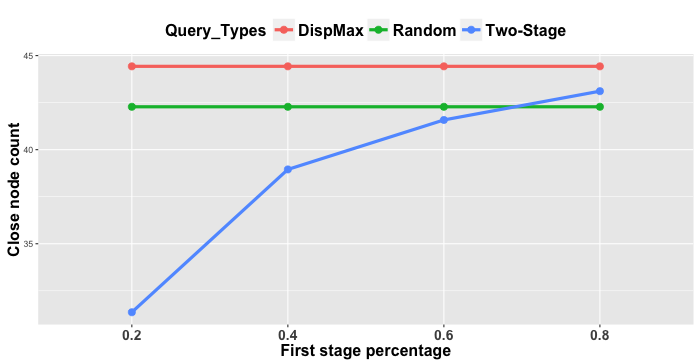
\includegraphics[width=9cm ,height=5.5cm]{figuresPng/Uni-Inc_Coverage.png}
\caption{Incident coverage for different values of First stage percentage. }
\label{fig:uniIncdCove}
\end{figure}
\subsection{Long tail distribution}
In this subsection, the incidents are generated according to a special case of the Long Tail distribution called the ``Pareto principle''. According to the Pareto principle, we assume that $20\%$ of the matrix cells are home for $80\%$ of the incidents while conversly $80\%$ of the matrix cells are home for $20\%$ of the incidents. We generate $100$ different matrices applying the Pareto Principle randomly on the cells. We use a random uniform distribution to select $20\%$ of the cells and generate $80\%$ of the incidents uniformly for these cells and vice versa. Figure~\ref{fig:LTClosePeople} shows that the two-stage outperforms both the random policy and the dispersion maximization policy by up to $10.2\%$ and $12.1\%$, respectively, in terms of close node count. This is due to the clustering of events in only $20\%$ of the grid which means that more than one incident is likely to occur in the same cell. So, if the two-stage technique reaches a node close to an incident in one cell, this same node will cover more than one incident in the same cell. Dispersion maximization achieves the best incident coverage as shown in Figure~\ref{fig:LTIncdCove}. The two- stage technique approaches the maximum incident coverage when $FSP = 80\%$ with a difference of $1.24$ incidents on average.
\begin{figure}[!h]
\centering
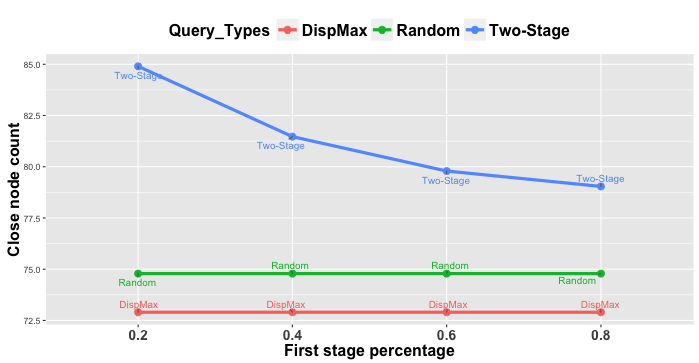
\includegraphics[width=9cm ,height=5.5cm]{figuresPng/LT-closePeople.png}
\caption{Close node count for different values of First stage percentage in the case of a long tail distribution. }
\label{fig:LTClosePeople}
\end{figure}
\begin{figure}[!h]
\centering
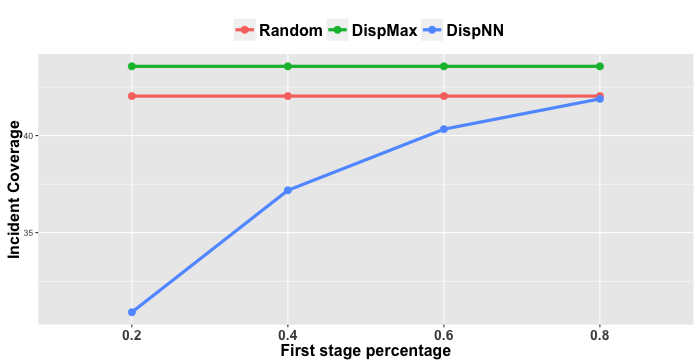
\includegraphics[width=9cm ,height=5.5cm]{figuresPng/LT-incidCov.png}
\caption{Incident coverage for different values of First stage percentage in the case of a long tail distribution. }
\label{fig:LTIncdCove}
\end{figure}
\subsection{Case study: Hollaback harassment data set}
After applying the two-stage querying technique to the previously mentioned three distributions (clustered, uniform and long-tail), we wish to examine the technique under real incident distributions. To do that, we test our querying technique on a global street harassment dataset provided by Hollaback~\cite{hollaback}.
\subsubsection{Data overview}
Hollaback is a non-profit movement powered by local activists in $92$ cities and $32$ countries to end street harassment. The Hollaback project collects data on street harassment events worldwide. Through the Hollaback phone app and the online platform, users can report stories of street harassment to share with the Hollaback community. This empowers victims to speak out about everyday harassment and spread the word about the prevalence of these events. In some communities, local governments are informed in real-time about street harassment so that there is a system-wide level of accountability. In addition, the Hollaback app uses GPS to record a data set that represents the locations of street harassment events as a means of improving the collective understanding of street harassment and how it can be prevented.  As of January $2016$, over $8000$ street harassment incidents have been recorded in their dataset since February $2011$.  It is on this data set that we wish to test the two-stage querying technique.\par
\subsubsection{Analysis}
From the Hollaback dataset, we select cities for which we have enough harassment samples for statistical significance (i.e. more than 30 samples). We test the performance of Random selection, Dispersion maximization selection, and the two-stage querying on six different cities: Paris, Brussels, Berlin, Baltimore, Buenos Aires and Istanbul. These cities were in the top ten cities with respect to the number of harassment reports in this dataset. In this paper, we show results for Paris, Brussels, and Istanbul. The results for Berlin, Baltimore, and Buenos Aires were consistent with the results shown in this paper. \par

As a first step, we must parse the Hollaback dataset such that incidents reports are grouped by city. To do so, we use bounding box coordinates. We then draw the border lines for the different cities and remove any outliers from our datasets. Figure~\ref{fig:citiesDistribution} shows the resulting distribution of events for the three-case study. \par
%The Paris dataset contains , while the Brussels dataset contains $154$ incidents covering a geographic area of $28.4$ $mi^2$. Istanbul has $87$ reported incidents covering an area of $138$ $mi^2$ on the left of the Bosporus Strait and $69$ $mi^2$ on the right. \par
\begin{figure}[!h]
\centering
\subcaptionbox{ Paris: $197$ harassment incidents and covering an area of $28.2$ $mi^2$. \label{fig: clust_20}}{%
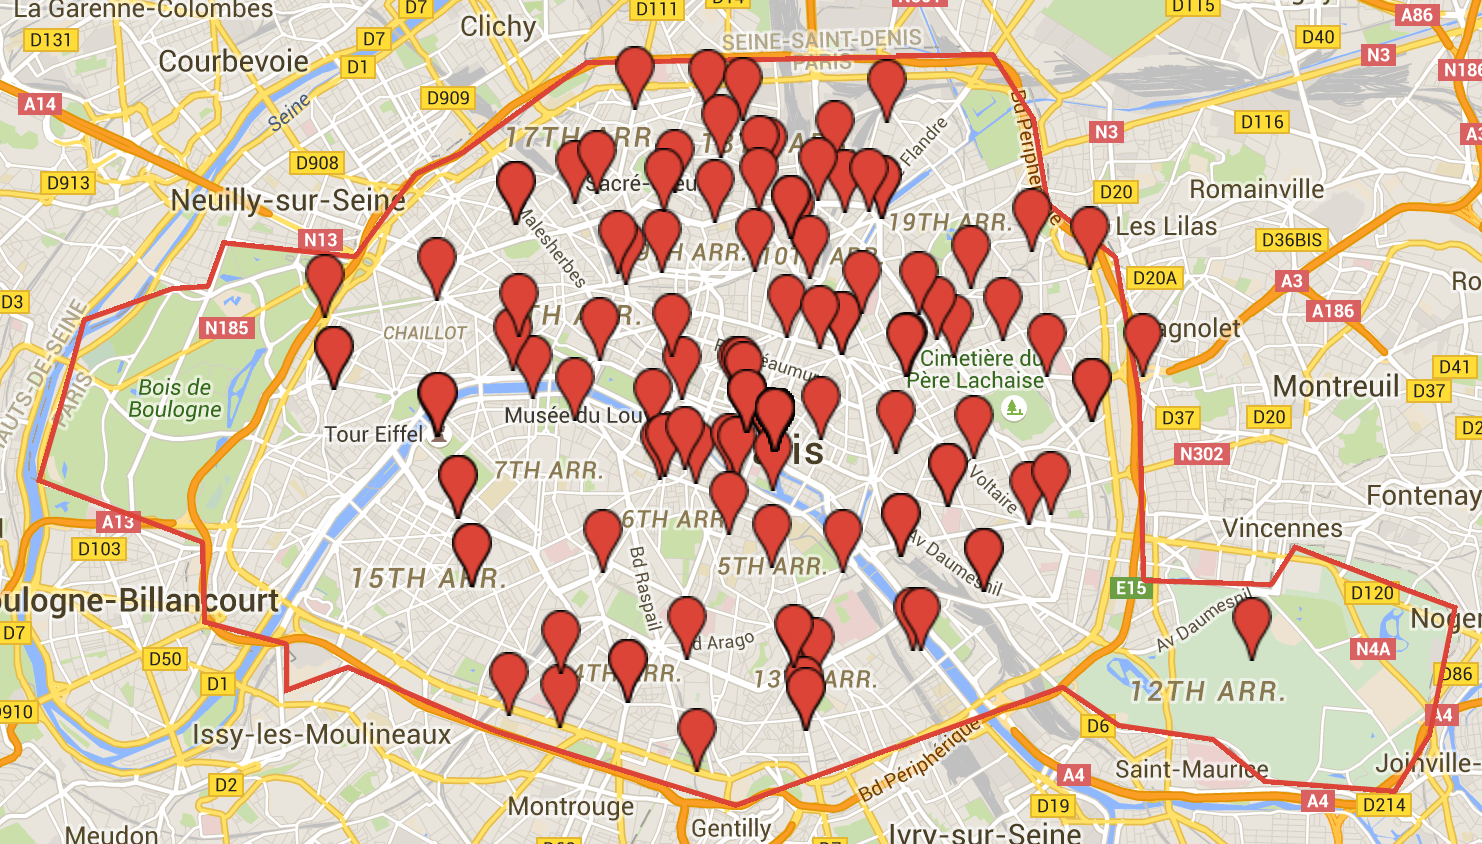
\includegraphics[width=8cm, height=5cm]{figuresPng/Paris.png}%
}\par\medskip
\subcaptionbox{Brussels: $154$ incidents covering an area of $28.4$ $mi^2$.\label{fig: clust_40}}{%
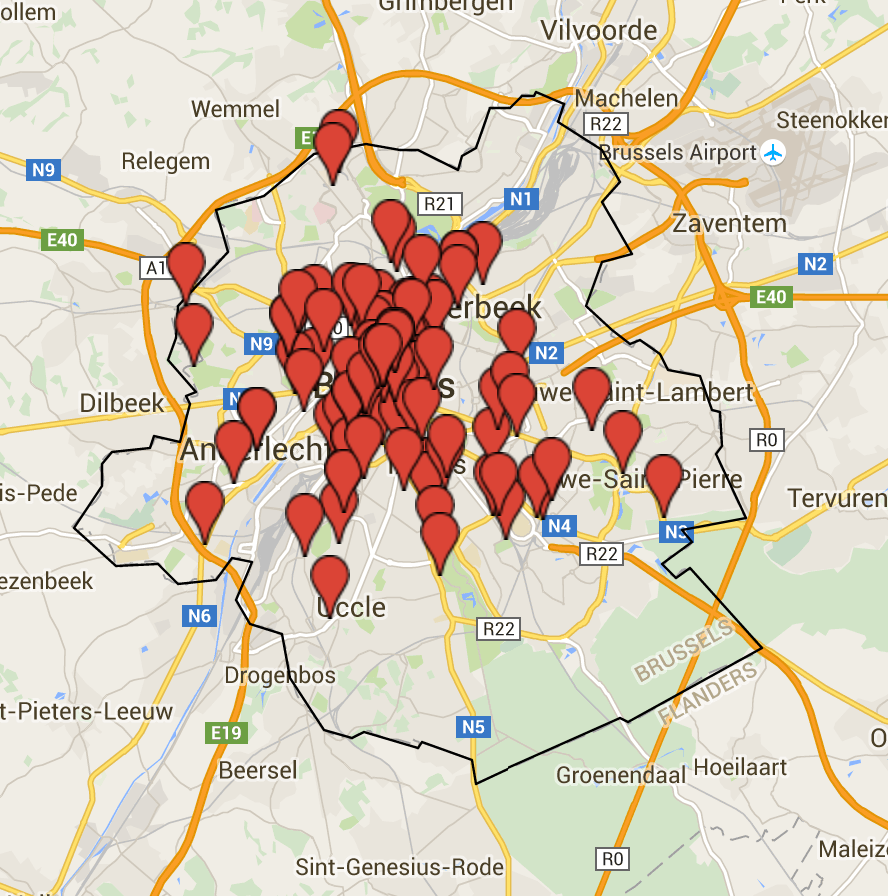
\includegraphics[width=8cm, height=5cm]{figuresPng/Brussels.png}%
}\par\medskip     
\subcaptionbox{ Istanbul: $87$ reported incidents covering an area of $138$ $mi^2$ on the left of the Bosporus Strait and $69$ $mi^2$ on the right.\label{fig: clust_60}}{%
  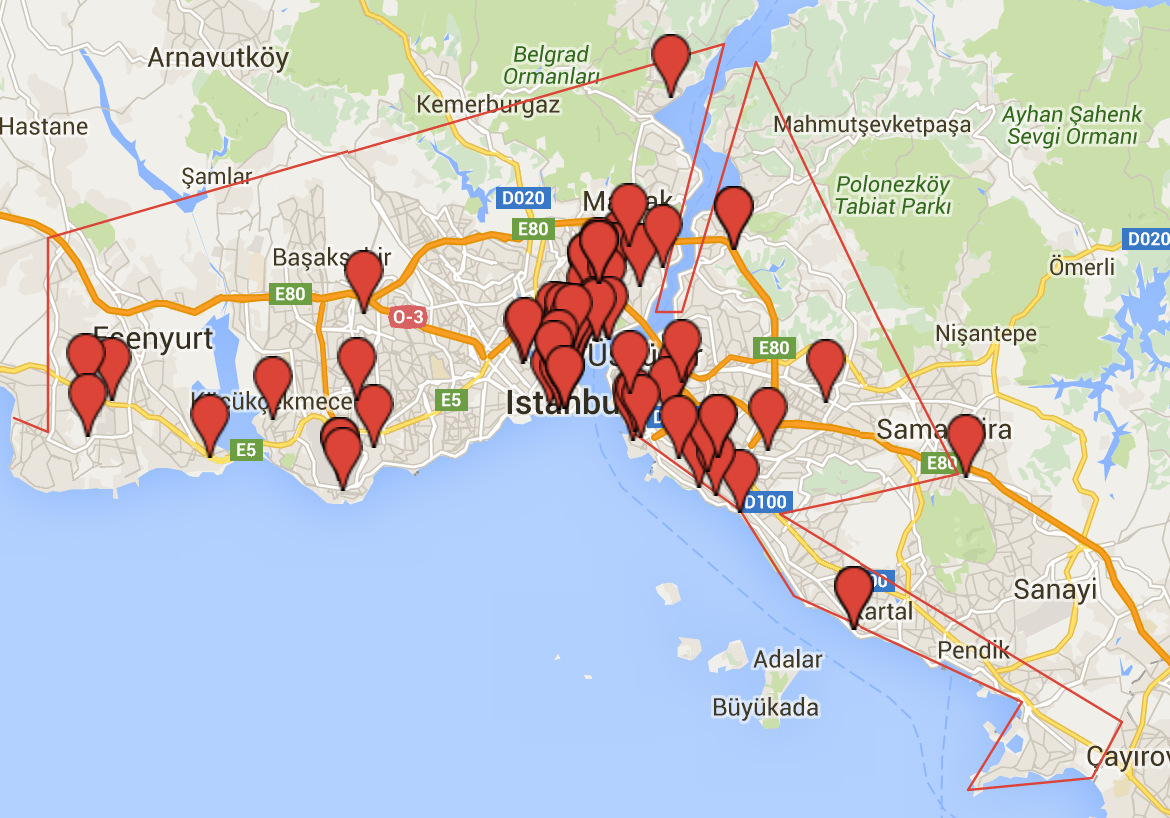
\includegraphics[width=8cm ,height=5cm]{figuresPng/Istanbul.png}%
}
\caption{Distribution of harassment incidents across representative city datasets.}
\label{fig:citiesDistribution}
\end{figure}
For each of the cities, we generate different variations of uniformly distributed crowds ($M = 100$) across the city. In this kind of analysis, the parameters, matrix dimension and incident count, are not generated by our analysis but rather taken from the dataset. In this case, we update the distance metric in Equation~\ref{eq:maxDisp} and use the Haversine formula to calculate the great-circle distance between two points as follows:
\begin{equation} \label{eq:maxDisp2}
d = 2R*atan2(\sqrt{a}, \sqrt{1-a})
\end{equation}
where $a$ is calculated as $ \sin ^2((\Delta \phi)/2 ) + \cos(\phi_1)\cos(\phi_2) * \sin ^2((\Delta \lambda)/2 )$, $\Delta \phi$ and $\Delta \lambda$ are calculated as the radian difference between the latitudes and longitudes, respectively, and $R$ is the Earth's radius (mean radius = 6,371km). We measure the Close node count and the Incident Coverage for all three querying techniques and plot the results in Figures~\ref{fig: hollaCloseCount} and~\ref{fig: hollaIncCoverage}, respectively. The Two-stage algorithm outperforms both the Random and Dispersion Maximization in terms of Close node count for all three cities. In terms of incident coverage, Figure~\ref{fig: hollaIncCoverage} shows that dispersion maximization achieves maximum incident coverage. The figure also shows that the two-stage technique can achieve this maximum by setting the first stage percentage to be $80\%$. Figures~\ref{fig: hollaCloseCount} and~\ref{fig: hollaIncCoverage} suggest that there is an inherent tradeoff between accuracy and coverage under constrained resources which we discuss in detail in later sections. The figures also suggest that the two-stage technique when the first stage percentage is $80\%$, can achieve a balance between accuracy and coverage.\par
\begin{figure}[!h]
\centering
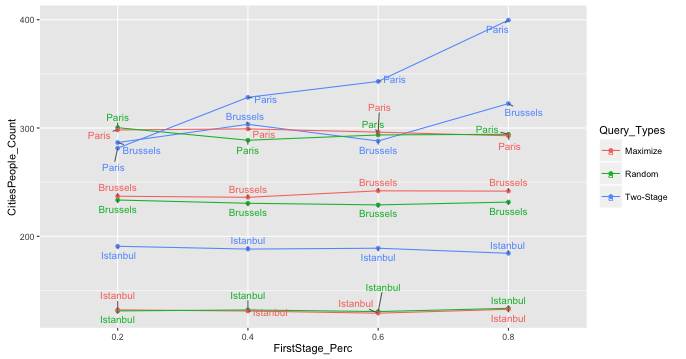
\includegraphics[width=9cm ,height=6cm]{figuresPng/hollaCloseCnt.png}
\caption{Close node count for different values of First stage percentage. }
\label{fig: hollaCloseCount}
\end{figure}
\begin{figure}[!h]
\centering
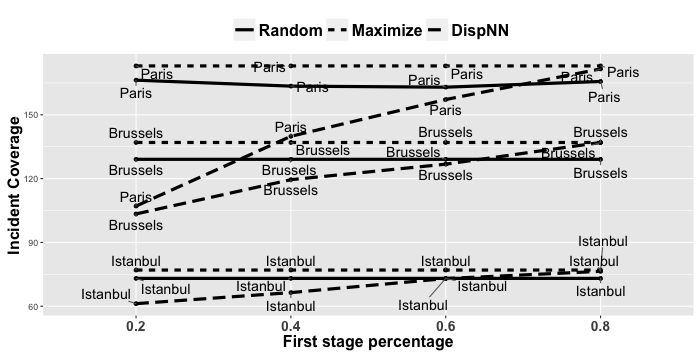
\includegraphics[width=9cm ,height=6cm]{figuresPng/citiesInc.png}
\caption{Incident coverage for different values of First stage percentage. }
\label{fig: hollaIncCoverage}
\end{figure}
\subsection{Stressing the two-stage querying algorithm (k=1)}
After applying the two-stage technique to different datasets, we are interested in checking which schemes were able to query nodes that were the first nearest neighbors to the incidents. This is beneficial, for example, when targeting first responders in an emergency scenario or in a spatial task distribution where you want to select the nearest neighbors to maximize spatial task assignment. This can be viewed as stressing the selection policies in order to determine which achieves a higher number of first nearest neighbors.\par

To study first nearest neighbors, we examine the Hollaback datasets for Paris, Brussels, and Istanbul. We examine the total close node count and for each incident, we determine whether we selected the first nearest neighbor in the queried users set. These results are shown in Table~\ref{table:NNParis}, where NN denotes nearest neighbors, CNC denotes close node count, and TS denotes the two-stage querying technique. For Paris, the two-stage technique achieves a $9.5\%$ surge on average in selecting nearest neighbors in comparison to dispersion maximization and $19\%$ surge in comparison to random selection. For Brussels (Bruss), the surge is $14.2\%$ and $21.35\%$ in comparison to dispersion maximization and random selection, respectively. For Istanbul (Istan), the surge percentages were $26.7\%$ and $36.5\%$.
\begin{table}[!h]
\centering
\begin{tabulary}{0.5\textwidth}{|C|C|C|C|C|C|C|}
\hline
City & Random & DispMax & TS ($FSP = 0.2$) & TS ($FSP = 0.4$)  & TS ($FSP = 0.6$)  &TS ($FSP = 0.8$)   \\ \hline
Paris-NN & $58$ & $63$  & $54$  & $69$ & $69$ & $84$  \\ \hline
Paris-CNC   & $300$ & $298$  & $281$  & $328$ & $343$ & $399$  \\ \hline
Bruss-NN & $48$ & $51$  & $55$  & $58$ & $55$ & $65$  \\ \hline
Bruss-CNC   & $233$ & $237$  & $286$  & $303$ & $288$ & $322$  \\ \hline
Istan-NN & $26$ & $28$  & $36$  & $37$ & $35$ & $36$  \\ \hline
Istan-CNC   & $131$ & $132$  & $190$  & $188$ & $188$ & $184$  \\ \hline
\end{tabulary}
\caption{First nearest neighbors (NN) count and close node count for Paris, Brussels, and Istanbul.}
\label{table:NNParis}
\end{table}
\section{Discussion}
\subsection{Tradeoff}
In the previous section, we examined the performance of the two-stage querying technique in a variety of incident and node/user configurations and we observed that as $FSP$ decreases, the close node count tends to increase. We also observed that in this case the same node can be in the K nearest neighbors for multiple incidents. This means that the algorithm tends to select central nodes that are in proximity with other incidents. This is beneficial in cases where the centrality of nodes is important to the problem, e.g. minimizing trip costs to these incidents and maximizing task assignments. This observation ensures diversity/accuracy of the feedback, i.e., instead of relying on a small number of nodes close to the incidents, we have a greater sample that can contribute to the measurement.
On the other hand, as $FSP$ increases so does the probability of catching more incidents in the spatial environment, which is crucial in applications where coverage is important and where a false positive is less expensive than a false negative. This is due to the fact that more nodes are selected in the first stage and fewer nodes in the second phase. It is no surprise, under resource constrained conditions, there is a tradeoff between accuracy and coverage.

\subsection{Technique variants}
\subsubsection{Trust-based responses}
In our second stage of our algorithm, we select users based on the pivot nodes that provide a positive feedback in the first stage. To incorporate trust into the algorithm, trust-based algorithms can provide feedback about certain nodes and their feedback. If some of the nodes queried in the first stage of the algorithm were deemed trust unworthy, the second stage can be divided into two querying steps. The first step is the KNN for the trustworthy-nodes, and the second is determining dispersion maximization. 
\subsubsection{Prior knowledge availability}
The two-stage querying technique does not assume any knowledge about the distribution of events. Given some prior information about the distribution, the algorithm can be tailored to take the prior distribution into account. The idea is to divide the spatial area into bounding regions and for each region we give a specific weight that reflects the probability of occurrence in that bounding regions.
For example, Figure~\ref{fig: BaltimoreRegions} shows Baltimore divided into four bounding regions denoted as br1, br2, br3, and br4. Using the knowledge that br3 has more incidents than br2, which has more incidents than br1 and br4, a higher weight should be given to br3. In particular, $br3_w > br2_w> br4_w> br1_w$ where the subscript $w$ denotes the weight assigned to the bounding region. The next step would be to apply the algorithm on the different bounding regions taking into account the weights assigned when allocation resources as shown in Algorithm~\ref{TSBR}.
\begin{algorithm}
\caption{Bounding regions two-stage variation.}
\label{TSBR}
 \begin{algorithmic}[1]
     \Function{selectUsersBRs }{$BRs[], w[], N, FSP$}
     \State selectedUsers = $\left\{\right\}$
      \State BRQuota = calculateQuota(BRs[], w[], N)
       \For{$br$ in BRs}
       \State brQuota = BRQuota(br)
     \State brUsers = selectUsersFromGrid(FSP, brQuota)
     \State brUsers.append(brUsers)
   \EndFor
\State return {selectedUsers}
\EndFunction
\end{algorithmic}
\end{algorithm}
\begin{figure}[!h]
\centering
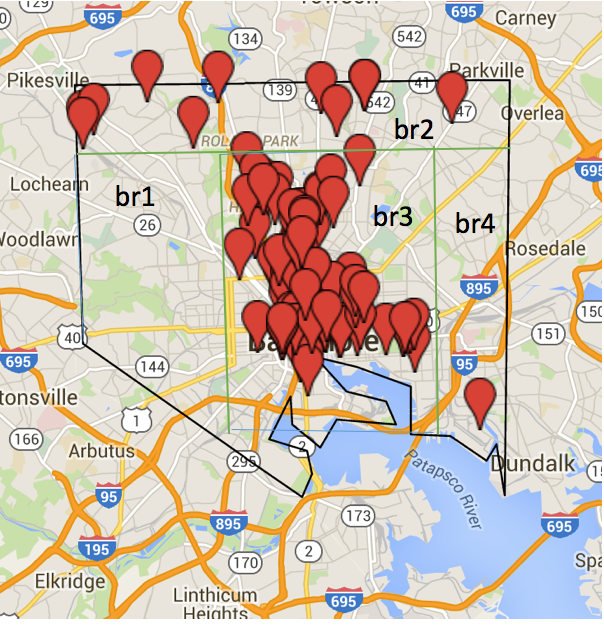
\includegraphics[width=9cm ,height=5.5cm]{figuresPng/BaltimoreBr.png}
\caption{Baltimore divided into bounding regions depending on prior knowledge of harassment occurrence.}
\label{fig: BaltimoreRegions}
\end{figure}
\section{Conclusion}
This paper proposed a two-stage spatial querying technique that attempts to probe nodes that are closer to the incidents in a $2D$ spatial environment. The algorithm maximizes the dispersion of location in the first stage and selects the K nearest neighbors in the second stage based on node feedback. The experimental evaluation confirms the applicability of proposed approach.
Important aspects that need to be taken into consideration include the sensing range and the sensing accuracy of the nodes. Nodes with accurate sensing and larger sensing ranges will provide more robustness to the two-stage technique. Another important parameter that can impact the performance of the technique is the distribution of the available nodes in the spatial environment. To ensure an optimal performance, nodes should be placed uniformly in the environment if the incident distribution is not known or following an approximate distribution of the incidents. The node placement can be controlled for some senors like traffic or agriculture sensors while in other cases it is hard to be controlled especially when human participation is involved. In that case, there are no gurantees that humans as sensors will be uniformly distributed across the spatial area under investigation. Another important factor when choosing the number of nodes to query is the granularity of the incidents. For instance, when using human as sensors, incidents such as disasters can likely be sensed/detected by numerous people in the range of the incident. On the other hand, incidents such as street harassment require the presence of the human at the same exact place of the incident; otherwise, the incident is unlikely to be detected.

\section{Acknowledgments}
The authors would like to thank Hollaback for sharing their collected dataset and taking the time to answer questions.
\bibliographystyle{abbrv}
{\footnotesize
\bibliography{sigproc}}  % sigproc.bib is the name of the Bibliography in this case
% You must have a proper ".bib" file
%  and remember to run:
% latex bibtex latex latex
% to resolve all references
%
% ACM needs 'a single self-contained file'!
%
%APPENDICES are optional
%\balancecolumns
\end{document}

